
%
% Beispieldokument für TU beamer theme
%
% v1.0: 12.10.2014
% 
\documentclass[xcolor={dvipsnames}]{beamer}
\usetheme{TU}

\usepackage{booktabs}
\usepackage{tabularx}
\usepackage{multirow}
% Macro to make entire row bold from https://tex.stackexchange.com/questions/309833/format-whole-row-of-table-as-bold
\newcommand\setrow[1]{\gdef\rowmac{#1}#1\ignorespaces}
\newcommand\clearrow{\global\let\rowmac\relax}
\clearrow

\title{LFQ: Online Learning of Per-flow Queuing Policies using Deep Reinforcement Learning}

%\author[M. Bachl et al.]{%
%	\underline{Maximilian Bachl}\email{maximilian.bachl@tuwien.ac.at} \and Fares Meghdouri \and Tanja Zseby \and Joachim Fabini
%}
\author[M. Bachl et al.]{%
	\underline{Maximilian Bachl}\email{maximilian.bachl@tuwien.ac.at} \and Joachim Fabini \and Tanja Zseby
}
\institute{%
	Technische Universität Wien, Vienna, Austria
}

%\session{XXXX \#}

%Kann angepasst werden, wie es beliebt. Entweder das Datum der Präsentation oder das Datum der aktuellen Präsentations-Version.
%\date[\the\day.\the\month.\the\year]{\today}
\newcommand{\mydate}{June 15, 2020}
\date[\mydate]{\mydate}

\begin{document}

\maketitle

\section{Introduction}

\begin{frame}{``Bufferbloat''}
  \begin{itemize}
  \item If queues in routers/switches too small: \textbf{Underutilization}
  \item \textbf{Solution:} Make queues very \textbf{large} for maximum throughput!
  \item \textbf{New problem:} Packets \textbf{wait} a long time (several seconds) in the queue: Bufferbloat
  \end{itemize}
\end{frame}

\begin{frame}{CoDel}{Active Queue Management against Bufferbloat}
  \begin{itemize}
  \item Moving time window of 100\,ms
  \item Queuing Delay \textbf{must be $<$ 5\,ms} once in each window
  \item Otherwise: Drop packet(s)
  \end{itemize}
\end{frame}

\begin{frame}{Fair Queuing}
  \begin{itemize}
  \item Separate each flow in separate queue
  \item No flow can ``steal'' bandwidth
  \item Popular implementation for Linux: \texttt{fq}
  \end{itemize}
  \pause
  \begin{alertblock}{Static buffer size:}
	Buffer often too large or too small 
  \end{alertblock}
\end{frame}

\begin{frame}{\texttt{fq\_codel}}{Combining fair queuing with CoDel}
  \begin{itemize}
  \item State-of-the-art
  \item Separate queues
  \item Each queue managed by CoDel
  \item Keeps each flow's queue $<$ 5\,ms
  \item Linux implementation: \texttt{fq\_codel}
  \pause
  \end{itemize}
  \begin{alertblock}{Inadequate interaction with Congestion Control:}
	\textit{Cubic} doesn't achieve full throughput or keeps standing queue 
  \end{alertblock}
\end{frame}

\section{Concept}

\begin{frame}{Buffer too large}
            \centering
  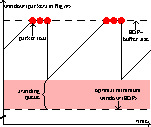
\includegraphics[height=0.9\textheight,keepaspectratio]{figures/cocoa_illustration_too_much.pdf}
\end{frame}

\begin{frame}{Buffer too small}
            \centering
  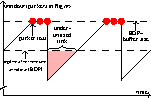
\includegraphics[height=0.9\textheight,keepaspectratio]{figures/cocoa_illustration_too_little.pdf}
\end{frame}

\begin{frame}{Buffer perfect}
            \centering
  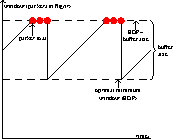
\includegraphics[height=0.9\textheight,keepaspectratio]{figures/cocoa_illustration_perfect.pdf}
\end{frame}

\begin{frame}{\texttt{cocoa} qdisc\footnote{\textit{Cocoa: Congestion Control Aware Queuing}, Bachl, Fabini, Zseby, 2020}}
\begin{itemize}
\item Fair queuing-based qdisc which \textbf{adapts} buffer \textbf{depending on congestion control}
\item Manages to achieve optimal throughput while keeping \textbf{delay} from buffering \textbf{minimal}
\item \textbf{Works} for common congestion controls
\end{itemize}
\pause
\begin{alertblock}{Hand-crafted algorithm:}
Works well for current congestion controls but might fail badly for new congestion controls.
\end{alertblock}
\end{frame}

\section{Concept}

\begin{frame}{Deep Learning for Buffering}
\begin{itemize}
\item Have a separate queue for each flow in a switch/router (fair queuing)
\item Define some reward function (like high throughput, low delay)
\item Use \textbf{Deep Learning}
\begin{itemize} \item to \textbf{fingerprint} each flow
\item and to use the \textbf{correct buffer size} for the flow \textbf{based on experience}, which \textbf{maximizes the reward}
\end{itemize}
\end{itemize}
\end{frame}

\begin{frame}{Reward}
\begin{align*}
\textit{Reward} = \textit{bandwidth}-\alpha\times\textit{queue size}
\end{align*}
\end{frame}

\begin{frame}{Input features}
\begin{itemize}
\item queue size
\item standard deviation of the queue size 
\item maximimum allowed buffer size
\item rate of incoming data
\item rate of outgoing data
\item time since the last packet loss
\end{itemize}
\end{frame}

\begin{frame}{Input features 2}
\begin{itemize}
\item Don't use these features themselves but exponentially weighted moving averages
\item Advantage: No need to keep data around except for features themselves
\end{itemize}
\end{frame}

\begin{frame}{Neural Network}
\begin{itemize}
\item It is a regression problem: Predict optimal buffer size for the flow based on the inputs
\item Fully connected neural network with three layers and leaky ReLU
\item Outputs optimal maximum buffer size each time packet is received
\begin{itemize}
\item To save compute it is possible, for example, only output optimum buffer size every 100\,ms
\end{itemize}
\end{itemize}
\end{frame}

\begin{frame}{Implementation}
\begin{itemize}
\item ns-3 for network simulation
\item Pytorch's C++ API for Deep Learning
\item Integrate Pytorch into ns-3
\item Develop queuing discipline based on fair queuing
\item Each flow is managed by Reinforcement Learning based on Deep Learning
\end{itemize}
\end{frame}

\section{Offline Learning}
\begin{frame}{Offline Learning}
\begin{itemize}
\item Randomly sample bandwidth, delay, congestion control and flow duration
\item For each flow, at random time, launch experiment
\item Experiment is A/B testing: 
\begin{itemize}
\item Continue with current buffer size +1 and current buffer size -1 (two different experiment)
\item Let the neural network learn buffer size that performed better regarding reward
\end{itemize}
\item Train using L1 loss (mean absolute error), using a couple of results together as a batch
\end{itemize}
Training takes several hundred thousand flows to converge. 
\end{frame}

\section{Offline Learning, $\alpha=0.01$}

\begin{frame}{Visualizing success}
Should learn
\begin{itemize}
\item Larger bandwidth $\rightarrow$ larger buffer
\item Larger delay $\rightarrow$ larger buffer
\end{itemize}
\end{frame}

%% Max: the following slide is probably too confusing...
%\begin{frame}{Offline training progress}
%\begin{figure}[h]
%\includegraphics[width=0.85\columnwidth]{{"figures/_mnt_cluster_results_RLQueueDisc_logs_plots_2020-6-6-10-24-18_prediction"}.png}
%\end{figure}
%\end{frame}

\begin{frame}{New Reno, varying bandwidth}
\centering
\includegraphics[width=0.85\columnwidth]{{"../ns-allinone-3.30.1/ns-3.30.1/results/RLQueueDisc/logs/plots/2020-6-6-10-24-18_81000.weights_New Reno_bandwidth"}.pdf}
\end{frame}

\begin{frame}{New Reno, varying delay}
\centering
\includegraphics[width=0.85\columnwidth]{{"../ns-allinone-3.30.1/ns-3.30.1/results/RLQueueDisc/logs/plots/2020-6-6-10-24-18_81000.weights_New Reno_delay"}.pdf}
\end{frame}

\begin{frame}{Bic, varying bandwidth}
\centering
\includegraphics[width=0.85\columnwidth]{{"../ns-allinone-3.30.1/ns-3.30.1/results/RLQueueDisc/logs/plots/2020-6-6-10-24-18_81000.weights_Bic_bandwidth"}.pdf}
\end{frame}

\begin{frame}{Bic, varying delay}
\centering
\includegraphics[width=0.9\columnwidth]{{"../ns-allinone-3.30.1/ns-3.30.1/results/RLQueueDisc/logs/plots/2020-6-6-10-24-18_81000.weights_Bic_delay"}.pdf}
\end{frame}

\begin{frame}{Correlations}
Correlations calculated of each of the above plots:\\ 
Correlation of 100\% $\rightarrow$ Our Reinforcement Learning system learned successfully
\begin{table}[h]
\caption{Correlation between bandwidth/delay of the link and output buffer size.} \label{tab:corrOfflineSmallAlpha}
\centering
\begin{tabular}{lrr} \toprule
Congestion control & bandwidth & delay \\ \midrule
New Reno & 98.3\% & 99.1\% \\
BIC & 80.2\% & 90.2\% \\
\bottomrule
\end{tabular}
\end{table}
\end{frame}

\begin{frame}{Average queue sizes}
Average queue is smaller for New Reno: This is expected since it has a larger multiplicative decrease parameter! \\
$\rightarrow$ New Reno needs a larger buffer on average so that the buffer never becomes empty. Our mechanism learned that!
\begin{table}[h]
%\caption{The average maximum queue length (in packets) output by the neural network after offline learning (tradeoff $0.01$) when averaging over flows with varying bandwidth/delay like in \autoref{tab:corrOfflineSmallAlpha}.} \label{tab:avgOfflineSmallAlpha}
\centering
\begin{tabular}{lr} \toprule
Congestion control & avg.~max.~queue length \\ \midrule
New Reno & 22 \\
BIC & 8 \\
\bottomrule
\end{tabular}
\end{table}
\end{frame}

\begin{frame}{25\,Mbit/s, 15\,ms, New Reno, LFQ}
\begin{figure}[h]
\includegraphics[width=0.85\columnwidth]{{"figures/local_ns-allinone-3.30.1_ns-3.30.1_results_RLQueueDisc_queueTraces_2020-6-6-10-24-18_81000.weights_cc_0_bw_25.000000_delay_15.000000"}.pdf}
%\caption{New Reno flow controlled by LFQ (offline training, $\alpha=0.01$); link speed: 25\,Mbit/s; delay: 15\,ms. The queue never becomes empty and also never forms a standing queue.}
\label{fig:exampleRenoLargeBw}
\end{figure}
\end{frame}

\begin{frame}{6\,Mbit/s, 15\,ms, New Reno, LFQ}
\begin{figure}[h]
\includegraphics[width=0.85\columnwidth]{{"figures/local_ns-allinone-3.30.1_ns-3.30.1_results_RLQueueDisc_queueTraces_2020-6-6-10-24-18_81000.weights_cc_0_bw_6.010101_delay_15.000000"}.pdf}
%\caption{Showing the maximum queue length and queue length of a New Reno flow controlled by LFQ (offline training, $\alpha=0.01$) at the bottleneck with a 6\,Mbit/s link and a delay of 15\,ms. The queue never becomes empty and also never forms a standing queue.}
\label{fig:exampleRenoSmallBw}
\end{figure}
\end{frame}

\begin{frame}{25\,Mbit/s, 15\,ms, BIC, LFQ}
\begin{figure}[h]
\includegraphics[width=0.85\columnwidth]{{"figures/local_ns-allinone-3.30.1_ns-3.30.1_results_RLQueueDisc_queueTraces_2020-6-6-10-24-18_81000.weights_cc_1_bw_25.000000_delay_15.000000"}.pdf}
%\caption{BIC flow controlled by \gls{ours} (offline training, $\alpha=0.01$); link speed: 25\,Mbit/s; delay: 15\,ms. The queue never becomes empty and also never forms a standing queue.}
\label{fig:exampleBicLargeBw}
\end{figure}
\end{frame}

\section{Offline Learning, $\alpha=10$}

\begin{frame}{Correlations}
\begin{table}[h]
\caption{Correlation between bandwidth/delay of the link and output buffer size.} \label{tab:corrOfflineSmallAlpha}
\centering
\begin{tabular}{lrr} \toprule
Congestion control & bandwidth & delay \\ \midrule
New Reno & 99.3\% & 96.5\% \\
BIC & 75.4\% & 62\% \\
\bottomrule
\end{tabular}
\end{table}
\end{frame}

\begin{frame}{Average queue sizes}
\begin{table}[h]
%\caption{The average maximum queue length (in packets) output by the neural network after offline learning (tradeoff $0.01$) when averaging over flows with varying bandwidth/delay like in \autoref{tab:corrOfflineSmallAlpha}.} \label{tab:avgOfflineSmallAlpha}
\centering
\begin{tabular}{lr} \toprule
Congestion control & avg.~max.~queue length \\ \midrule
New Reno & 13 \\
BIC & 5 \\
\bottomrule
\end{tabular}
\end{table}
\end{frame}

\begin{frame}{6\,Mbit/s, 15\,ms, New Reno, LFQ}
\begin{figure}[h]
\includegraphics[width=0.85\columnwidth]{{"figures/local_ns-allinone-3.30.1_ns-3.30.1_results_RLQueueDisc_queueTraces_2020-6-4-15-39-25_108000.weights_cc_0_bw_6.010101_delay_15.000000"}.pdf}
%\caption{Showing the maximum queue length and queue length of a New Reno flow controlled by LFQ (offline training, $\alpha=10$) at the bottleneck with a 6\,Mbit/s link and a delay of 15\,ms. The queue occasionally becomes empty which is intended as with the higher tradeoff $\alpha$, LFQ tries to favor a small queue more than high throughput.}
\label{fig:exampleRenoSmallBwLargeAlpha}
\end{figure}
\end{frame}

\section{Online Learning, $\alpha=10$}

\begin{frame}{Online Learning}
Same as Offline Learning except:
\begin{itemize}
\item Don't do A/B testing
\item Instead: Use second neural network that outputs expected reward (\textit{Critic Network}) (trained using L2 loss (mean squared error).
\item Either perform experiment A \textbf{or} experiment B (either current buffer size -1 packet or +1 packet)
\item If result was better than what the Critic Network expected, let first neural network (\textit{Actor Network}) learn to output this buffer size in the future.
\end{itemize}
Training takes longer (several million training flows)
\end{frame}

%% Max: the following slide is probably too confusing...
%\begin{frame}{Online training progress}
%\begin{figure}[h]
%\includegraphics[width=0.85\columnwidth]{{"figures/_mnt_cluster_results_RLQueueDisc_logs_plots_2020-6-1-16-41-30_prediction"}.png}
%\end{figure}
%\end{frame}

\begin{frame}{Correlations}
\begin{table}[h]
\caption{Correlation between bandwidth/delay of the link and output buffer size.} \label{tab:corrOfflineSmallAlpha}
\centering
\begin{tabular}{lrr} \toprule
Congestion control & bandwidth & delay \\ \midrule
New Reno & 86.1\% & 87.7\% \\
BIC & 72.9\% & 73.6\% \\
\bottomrule
\end{tabular}
\end{table}
\end{frame}

\begin{frame}{Average queue sizes}
\begin{table}[h]
%\caption{The average maximum queue length (in packets) output by the neural network after offline learning (tradeoff $0.01$) when averaging over flows with varying bandwidth/delay like in \autoref{tab:corrOfflineSmallAlpha}.} \label{tab:avgOfflineSmallAlpha}
\centering
\begin{tabular}{lr} \toprule
Congestion control & avg.~max.~queue length \\ \midrule
New Reno & 14 \\
BIC & 8 \\
\bottomrule
\end{tabular}
\end{table}
\end{frame}

\section{Comparison}

\begin{frame}{Example: Our solution}{15\,Mbit/s bandwidth, 5\,ms delay}
\begin{figure}[h]
\includegraphics[width=0.85\columnwidth]{{"figures/local_ns-allinone-3.30.1_ns-3.30.1_results_RLQueueDisc_queueTraces_2020-6-6-10-24-18_81000.weights_cc_1_bw_15.000000_delay_5.000000"}.pdf}
\end{figure}
\end{frame}

\begin{frame}{Example: FqCoDel (default on home routers)}{15\,Mbit/s bandwidth, 5\,ms delay}
\begin{figure}[h]
\includegraphics[width=0.85\columnwidth]{{"figures/local_ns-allinone-3.30.1_ns-3.30.1_results_FqCoDelQueueDisc_queueTraces_normal_cc_1_bw_15.000000_delay_5.000000"}.pdf}
\end{figure}
\end{frame}

\begin{frame}{Example: Fifo (default on Linux)}{\\ 15\,Mbit/s bandwidth, 5\,ms delay}
\begin{figure}[h]
\includegraphics[width=0.85\columnwidth]{{"figures/local_ns-allinone-3.30.1_ns-3.30.1_results_FifoQueueDisc_queueTraces_100_cc_1_bw_15.000000_delay_5.000000"}.pdf}
\end{figure}
\end{frame}

\begin{frame}{Systematic comparison}
\begin{table}
\caption{400 experiments; delay 5 -- 25\,ms; bandwidth 5 -- 25\,Mbit/s; New Reno and Bic Congestion Control. Results averaged.} \label{tab:comparison_others}
\centering
\begin{tabular}{l r r r} \toprule
& \multirow{2}{*}{avg. throughp.} & \multicolumn{2}{c}{queue size} \\
& & max. & avg. \\ \midrule
LFQ, offline $\alpha=0.01$ & 13.4 & 23.9 & 7.7\\
LFQ, offline $\alpha=10$ & 12.5 & 12.7 & 3.4\\
LFQ, online $\alpha=10$ & 12.8 & 16.1 & 4.5\\
FqCoDel	& 13.7 & 155.4 & 15.4\\
fq 100	& 11.7 & 100 & 51.1\\
fq 1000	& 11.9 & 1000 & 630.4 \\
\bottomrule
\end{tabular}
\end{table}
\end{frame}

\section{Discussion}

\begin{frame}{Observations}
\begin{itemize}
\item Scaling of features very important
\item Pytorch better to integrate with other code (ns-3) than TensorFlow
\item We thought simulating a flow in ns-3 would be faster than running it in the real world. It is not.
\end{itemize}
\end{frame}

\begin{frame}{Conclusion}
\begin{itemize}
\item LFQ is based on fair queuing
\item It fingerprints each flow
\item It learns to optimize a reward function
\item It achieves high throughput and low delay when compared to competing solutions
\item It has low computational overhead
\item We envision deployment close to end users (on switches, routers)
\end{itemize}
\end{frame}

%\begin{frame}{What could be improved}
%\begin{itemize}
%\item Behavior seems unstable sometimes
%\begin{itemize}
%\item Maybe lower training rate?
%\item Not L1 loss (mean absolute error) but L2 loss (mean squared error)? 
%\end{itemize}
%\item Online learning doesn't work for small $\alpha$. But is this really a problem?
%\end{itemize}
%\end{frame}

% -------------
% Last page
% -------------
\makelastslide

\end{document}